\documentclass[12pt,letterpaper]{article}
\usepackage[utf8]{inputenc}
\usepackage{tikz}
\usetikzlibrary{trees}
\usepackage[spanish, es-nodecimaldot]{babel}
\usepackage{amsmath}
\usepackage{color}
\usepackage{algorithm}
\usepackage[noend]{algpseudocode}
\renewcommand{\algorithmicrequire}{\textbf{Entrada:}}
\renewcommand{\algorithmicensure}{\textbf{Salida:}}
\usepackage{subcaption}
\usepackage{amsfonts}
\usepackage{hyperref}
 \hypersetup{
     colorlinks=true,
     linkcolor=blue,
     filecolor=blue,
     citecolor = blue,      
     urlcolor=cyan,
     }
\usepackage{amssymb}
\usepackage{listings}
\usepackage{color}

\definecolor{mygreen}{rgb}{0,0.6,0}
\definecolor{mygray}{rgb}{0.5,0.5,0.5}
\definecolor{mymauve}{rgb}{0.58,0,0.82}

\lstset{ 
  backgroundcolor=\color{white},   % choose the background color; you must add \usepackage{color} or \usepackage{xcolor}; should come as last argument
  basicstyle=\footnotesize,        % the size of the fonts that are used for the code
  breakatwhitespace=false,         % sets if automatic breaks should only happen at whitespace
  breaklines=true,                 % sets automatic line breaking
  captionpos=b,                    % sets the caption-position to bottom
  commentstyle=\color{mygreen},    % comment style
  deletekeywords={...},            % if you want to delete keywords from the given language
  escapeinside={\%*}{*)},          % if you want to add LaTeX within your code
  extendedchars=true,              % lets you use non-ASCII characters; for 8-bits encodings only, does not work with UTF-8
  firstnumber=1,                % start line enumeration with line 1000
  frame=single,	                   % adds a frame around the code
  keepspaces=true,                 % keeps spaces in text, useful for keeping indentation of code (possibly needs columns=flexible)
  keywordstyle=\color{blue},       % keyword style
  language=Octave,                 % the language of the code
  morekeywords={*,...},            % if you want to add more keywords to the set
  numbers=none,                    % where to put the line-numbers; possible values are (none, left, right)
  numbersep=5pt,                   % how far the line-numbers are from the code
  numberstyle=\tiny\color{mygray}, % the style that is used for the line-numbers
  rulecolor=\color{black},         % if not set, the frame-color may be changed on line-breaks within not-black text (e.g. comments (green here))
  showspaces=false,                % show spaces everywhere adding particular underscores; it overrides 'showstringspaces'
  showstringspaces=false,          % underline spaces within strings only
  showtabs=false,                  % show tabs within strings adding particular underscores
  stepnumber=2,                    % the step between two line-numbers. If it's 1, each line will be numbered
  stringstyle=\color{mymauve},     % string literal style
  tabsize=2,	                   % sets default tabsize to 2 spaces
  title=\lstname                   % show the filename of files included with \lstinputlisting; also try caption instead of title
}

\usepackage{amsthm}
\newtheorem{theorem}{Teorema}

\usepackage{graphicx}
\usepackage[inner=1.5 cm, outer = 1.5 cm, top=1 cm, bottom = 1.5 cm]{geometry}
\setlength{\parskip}{3mm}
\title{\textsc{Práctica 11: Frentes de Pareto}}
\author{\textsc{Fabiola Vázquez}}
\renewcommand{\lstlistingname}{Código}
\setlength{\parindent}{0cm}

\begin{document}
\maketitle

\hrule
\section{Introducción}
En esta práctica \cite{elisapractica10} se trabaja con optimización multicriterio, es decir, a un mismo conjunto de variables se le asignan valores de tal manera que se optimicen más de dos funciones objetivo, sin que una mejora de una función empeore otra. Primero se generan polinomios pseudo aleatorios y se determina si se va a minimizar o maximizar. Se trabaja con el concepto de dominancia de Pareto, se identifican todas aquellas soluciones que dominan (mejora por lo menos un objetivo sin empeorar ningún otro) y a dicho conjunto de soluciones se le denomina frente de Pareto. El objetivo de esta práctica es visualizar el porcentaje de soluciones que pertenecen al frente al ir aumentando la cantidad de funciones objetivo. El experimento se lleva a cabo en el software R \cite{R} en un cuaderno de Jupyter \cite{jupyter}.

\section{Experimento}
Se varía la cantidad $n$ de funciones, $n \in \{2,3,\ldots,12\}$. Para cada uno de los valores se realizan 200 repeticiones considerando la generación de 200 soluciones pseudo aleatorias. Los resultados se almacenan en un \texttt{data.frame}, el cuadro \ref{data} muestra un fragmento de los datos recopilados.

En la figura \ref{im} se tiene un gráfico comparando el porcentaje de soluciones que pertenecen al frente de Pareto para cada cantidad de funciones. Como se puede apreciar en dicha figura, al considerar cinco o más funciones el porcentaje de soluciones pertenecientes al frente es mayor que el 50\% y con siete o más se considera casi la totalidad de las soluciones como parte del frente. 

Se realiza pruebas T de Student para concluir si existen diferencia significativa entre las medias de cada uno de los conjuntos de datos. Como en la figura \ref{im} se aprecia que el porcentaje va en aumento, se realiza la prueba con grupos consecutivos. Se identifica a los conjuntos de números con la cantidad de funciones objetivos con las que se trabaja. En el cuadro \ref{p} se muestran los valores $p$ obtenidos en dichas pruebas. Como se puede apreciar en las primeras cinco pruebas se obtienen valores menores a 0.05, por lo que se concluye que sí existen diferencias significativas entre las medias. A partir de la prueba seis, los valores obtenidos son mayores que 0.05, por lo que no se tiene evidencia suficiente para considerar que existe una diferencia significativa entre dichos conjuntos.

 \begin{figure}
 	\centering 
		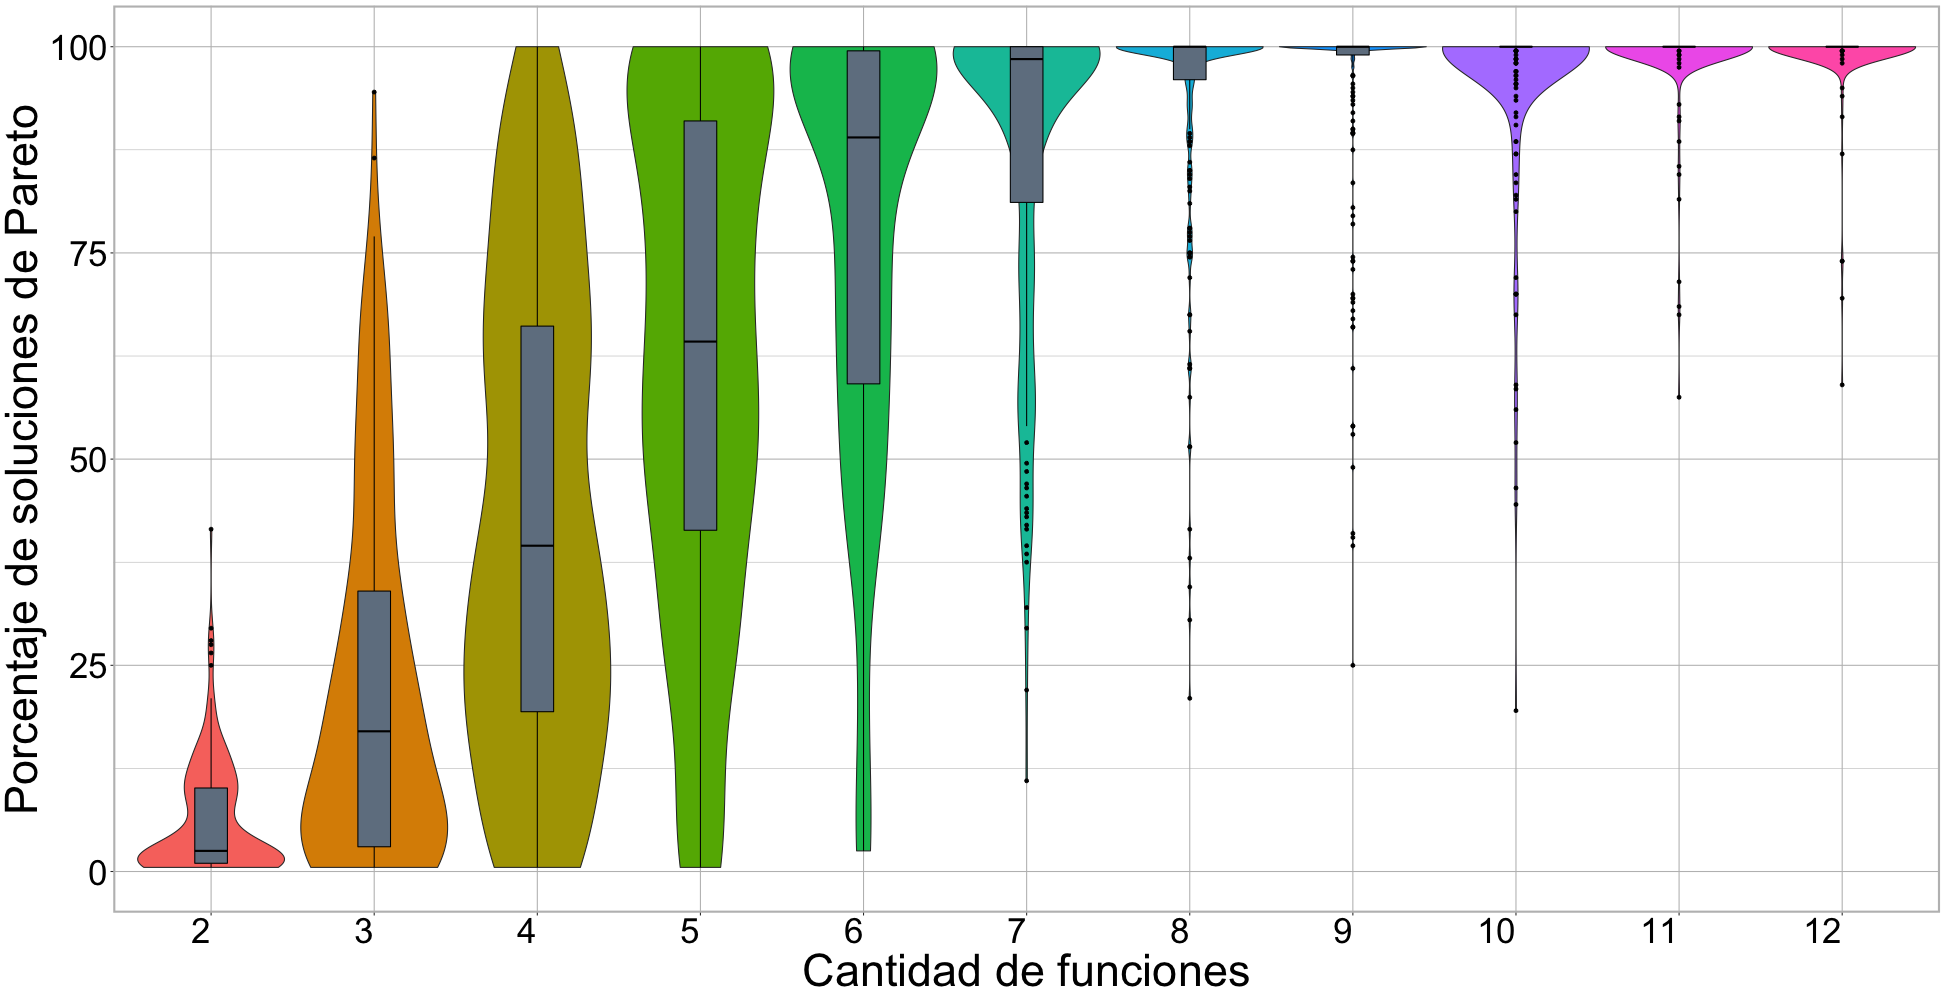
\includegraphics[width=\linewidth]{prueba2.png} 		
		\caption{Gráficos de violín del porcentaje de soluciones que son parte del frente de Pareto.}
		 		\label{im}
 	\end{figure}  




\begin{table}
\centering
\caption{Fragmento de los datos.}
\begin{tabular}{rr}
  \hline
Funciones & Porcentaje \\ 
  \hline
2 & 8.0 \\
3 & 24.0\\
4 & 1.0 \\
5 & 1.0 \\
6 & 57.0 \\
7 & 99.0 \\
8 & 99.5 \\
9 & 100.0\\
10 & 100.0\\
11 & 100.0\\
\hline
\end{tabular}
\label{data}
\end{table}

\begin{table}
\centering
\caption{Valores $p$ obtenidos de aplicar la prueba T de Student a distintos pares de conjuntos.}
\begin{tabular}{lr}
  \hline
Conjuntos & Valor $p$ \\ 
  \hline
2 y 3& $2.00\times 10^{-16}$ \\
3 y 4 & $1.18 \times 10^{-14}$\\
4 y 5 & $1.53 \times 10^{-06} $ \\
5 y 6 & $1.18 \times 10^{-05} $ \\
6 y 7 & $1.18 \times 10^{-04} $ \\
7 y 8 & $0.46$ \\
8 y 9 & 0.18 \\
9 y 10 & 0.03\\
10 y 11 & 0.50\\

\hline
\end{tabular}
\label{p}
\end{table}

\section{Reto 1}
En el primer reto se selecciona un subconjunto, cuyo tamaño es un porcentaje del tamaño del frente de Pareto de tal forma que el subconjunto esté \textit{diversificado}, es decir, que no esté agrupado en una sola zona del frente. En la figura \ref{1} se muestra un subconjunto del frente con el 50\% del tamaño original no diversificado, como se aprecia todas las soluciones se ubican en la zona inferior izquierda, a diferencia de la figura \ref{2} donde las soluciones están diversificadas.

Para lograr obtener el subconjunto diversificado, se trabaja con la función \texttt{kmeans} \cite{kmeans} que agrupa datos minimizando la distancia entre ellos. Esta función indica a que grupo pertenece cada dato, para tomar solo uno de cada grupo se utiliza la función de diversificación dada en el código \ref{lst:function}.

\begin{lstlisting}[caption = Función de diversificación., label={lst:function}]
diversidad <- function(front, porcentaje){
contador <- c()
posiciones <-c()
kmeans <- kmeans(front, round(dim(front)[1]*porcentaje/100), iter.max = 1000, nstart = 10)
for (i in 1:length(kmeans$cluster)){
    if(sum(kmeans$cluster[i]==contador)==0){
        posiciones <- c(posiciones, i)
        contador <- c(contador, kmeans$cluster[i])
    }
    
}
    return(posiciones)
    }
\end{lstlisting}

 \begin{figure}
 	\centering 
 	\begin{subfigure}[b]{0.47\linewidth}
 		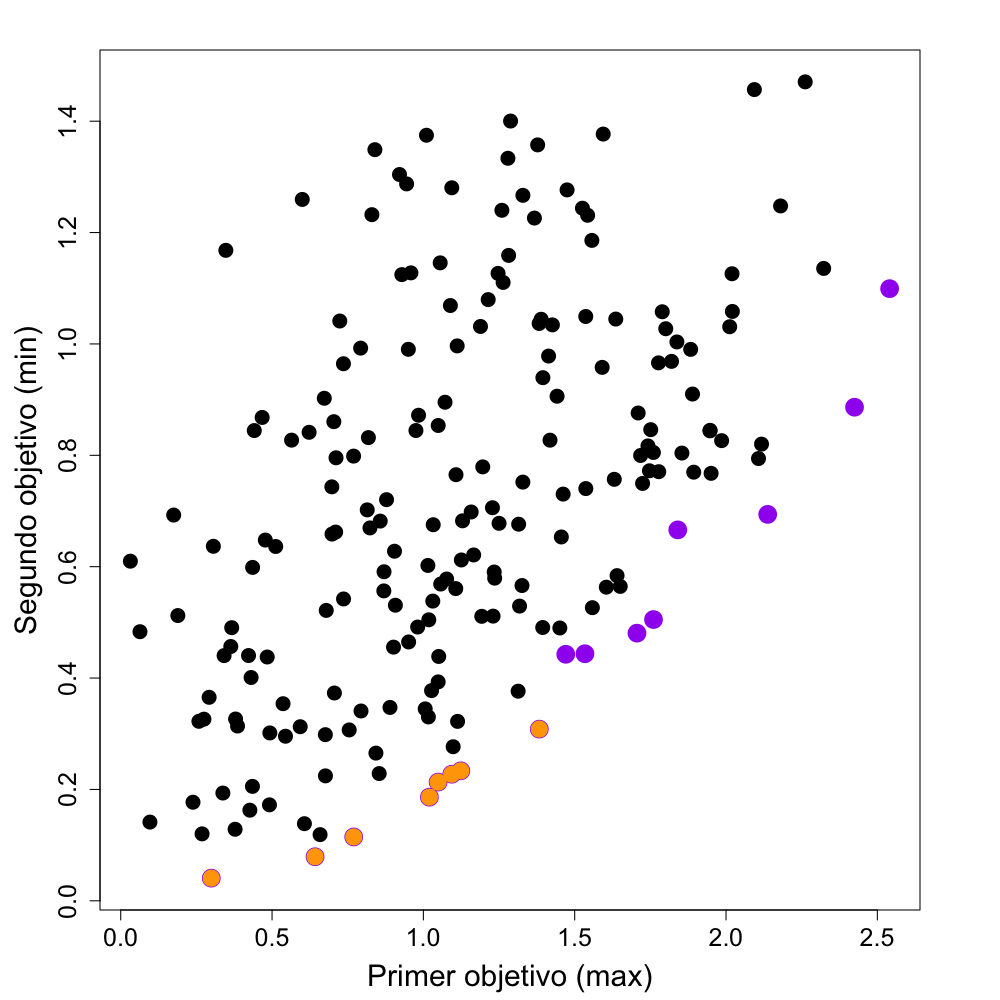
\includegraphics[width=\linewidth]{nodiv.png} 		
 		\caption{No diversificada.}
 		 		\label{1}
 	\end{subfigure}  \hfill
 	\begin{subfigure}[b]{0.47\linewidth}
 		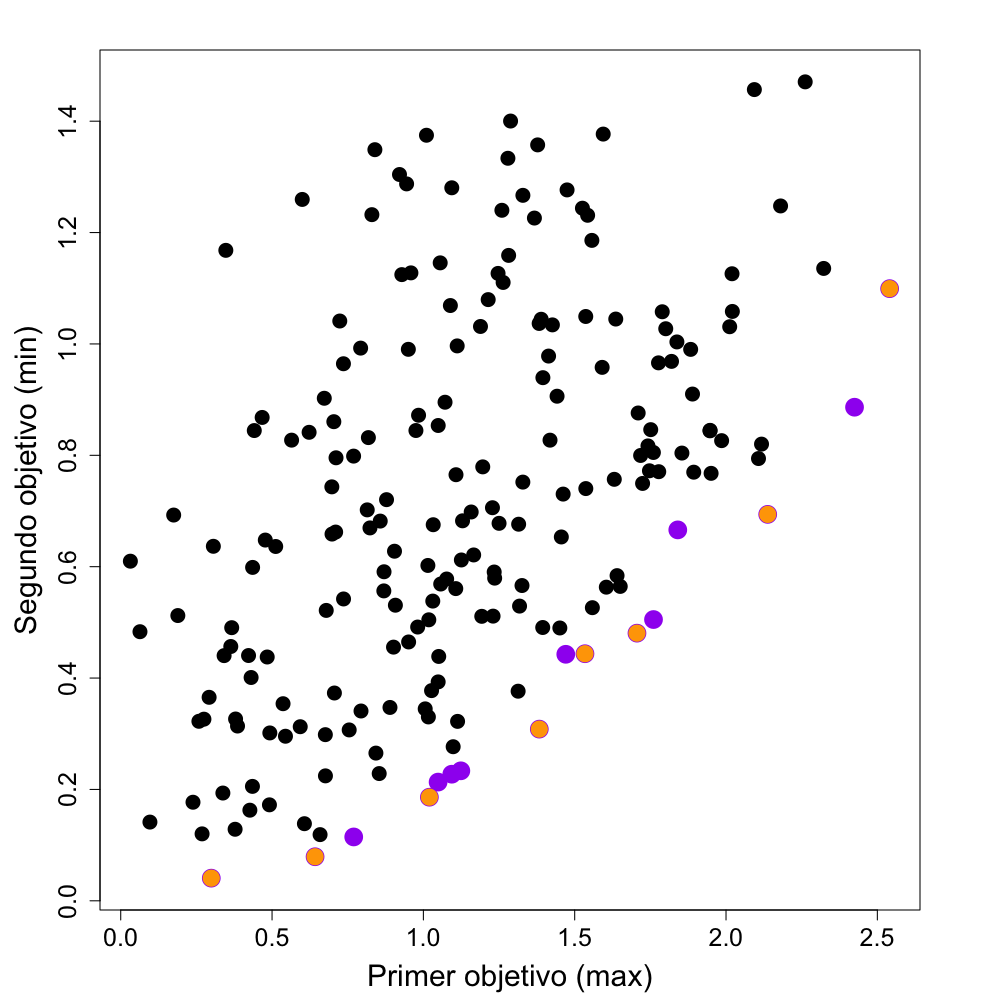
\includegraphics[width=\linewidth]{div.png} 		
 		\caption{Diversificada.}
 		\label{2}
 	\end{subfigure} 
 	 	\label{ex}
 	\caption{Ejemplos de subconjuntos (naranja) del frente de Pareto (morado).}
\end{figure} 

\begin{figure}
 	\centering 
 	\begin{subfigure}[b]{0.3\linewidth}
 		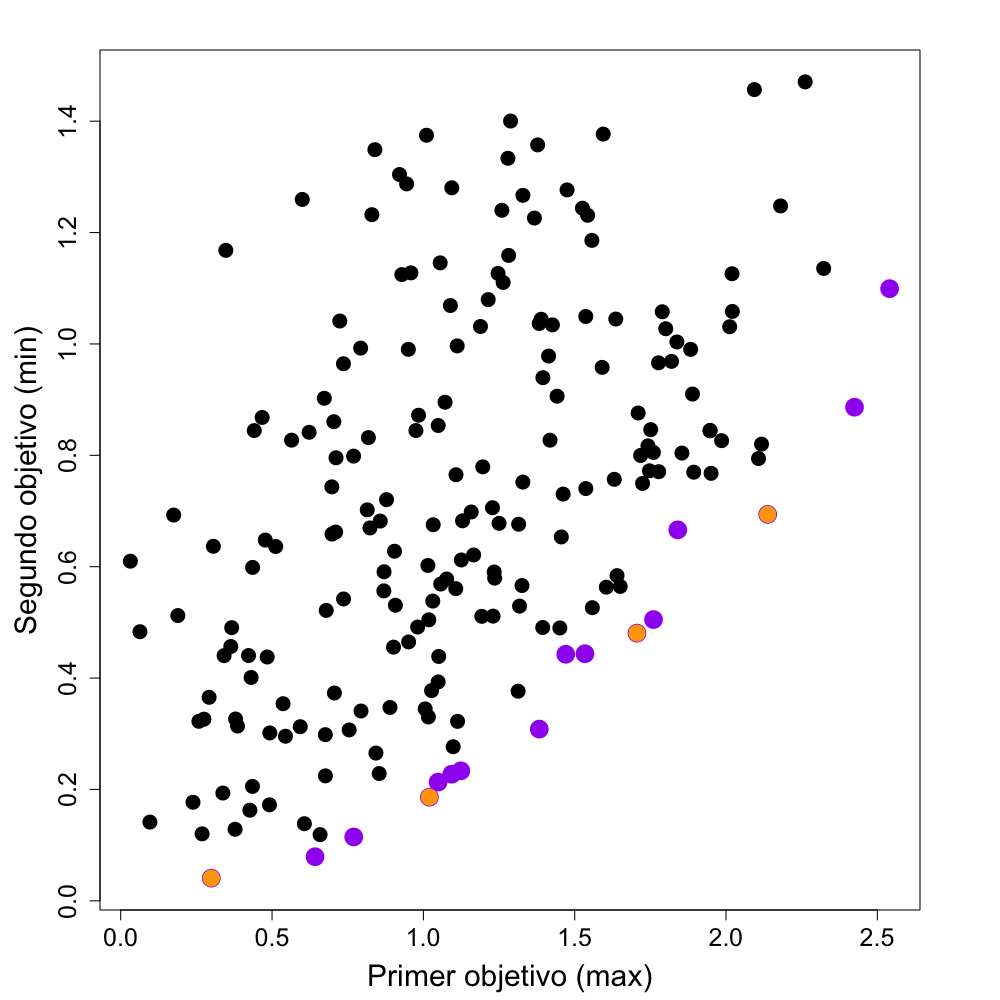
\includegraphics[width=\linewidth]{25.png} 		
 		\caption{Subconjunto con el 25\% del frente original.}
 		 		\label{25}
 	\end{subfigure}  \hfill
 	\begin{subfigure}[b]{0.3\linewidth}
 		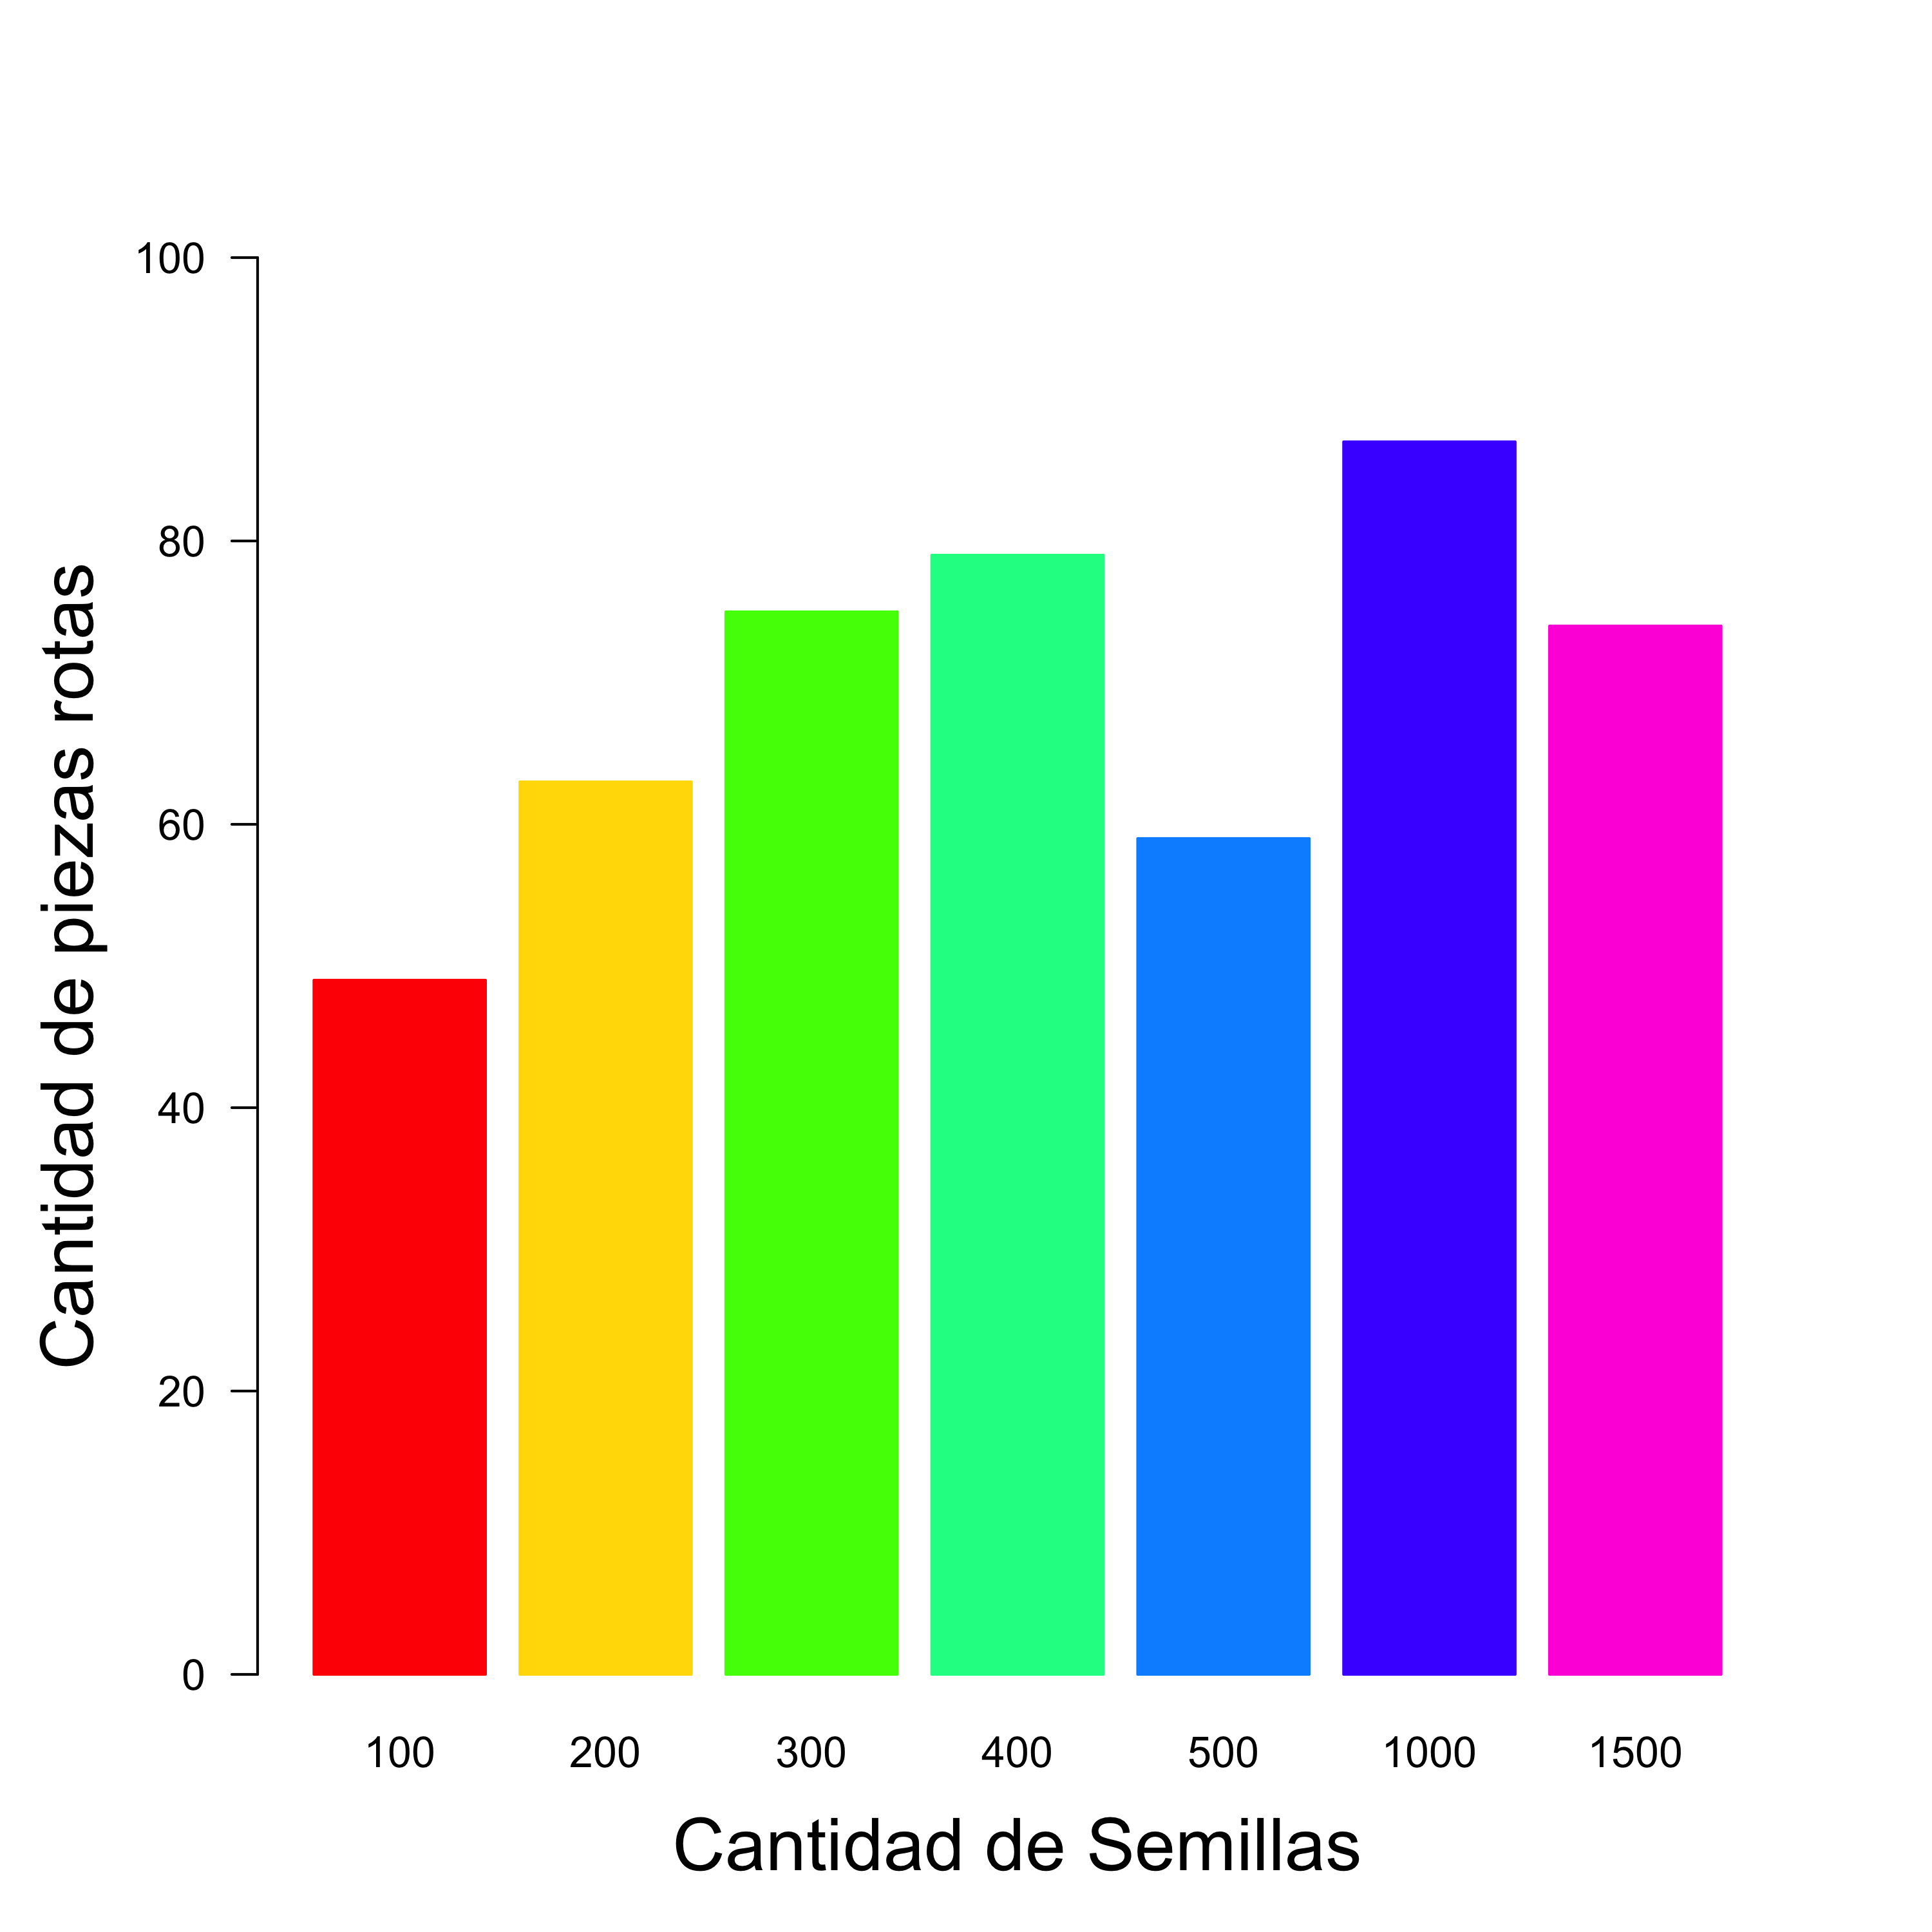
\includegraphics[width=\linewidth]{50.png} 		
 		\caption{Subconjunto con el 50\% del frente original.}
 		\label{50}
 	\end{subfigure} \hfill
 	\begin{subfigure}[b]{0.3\linewidth}
 		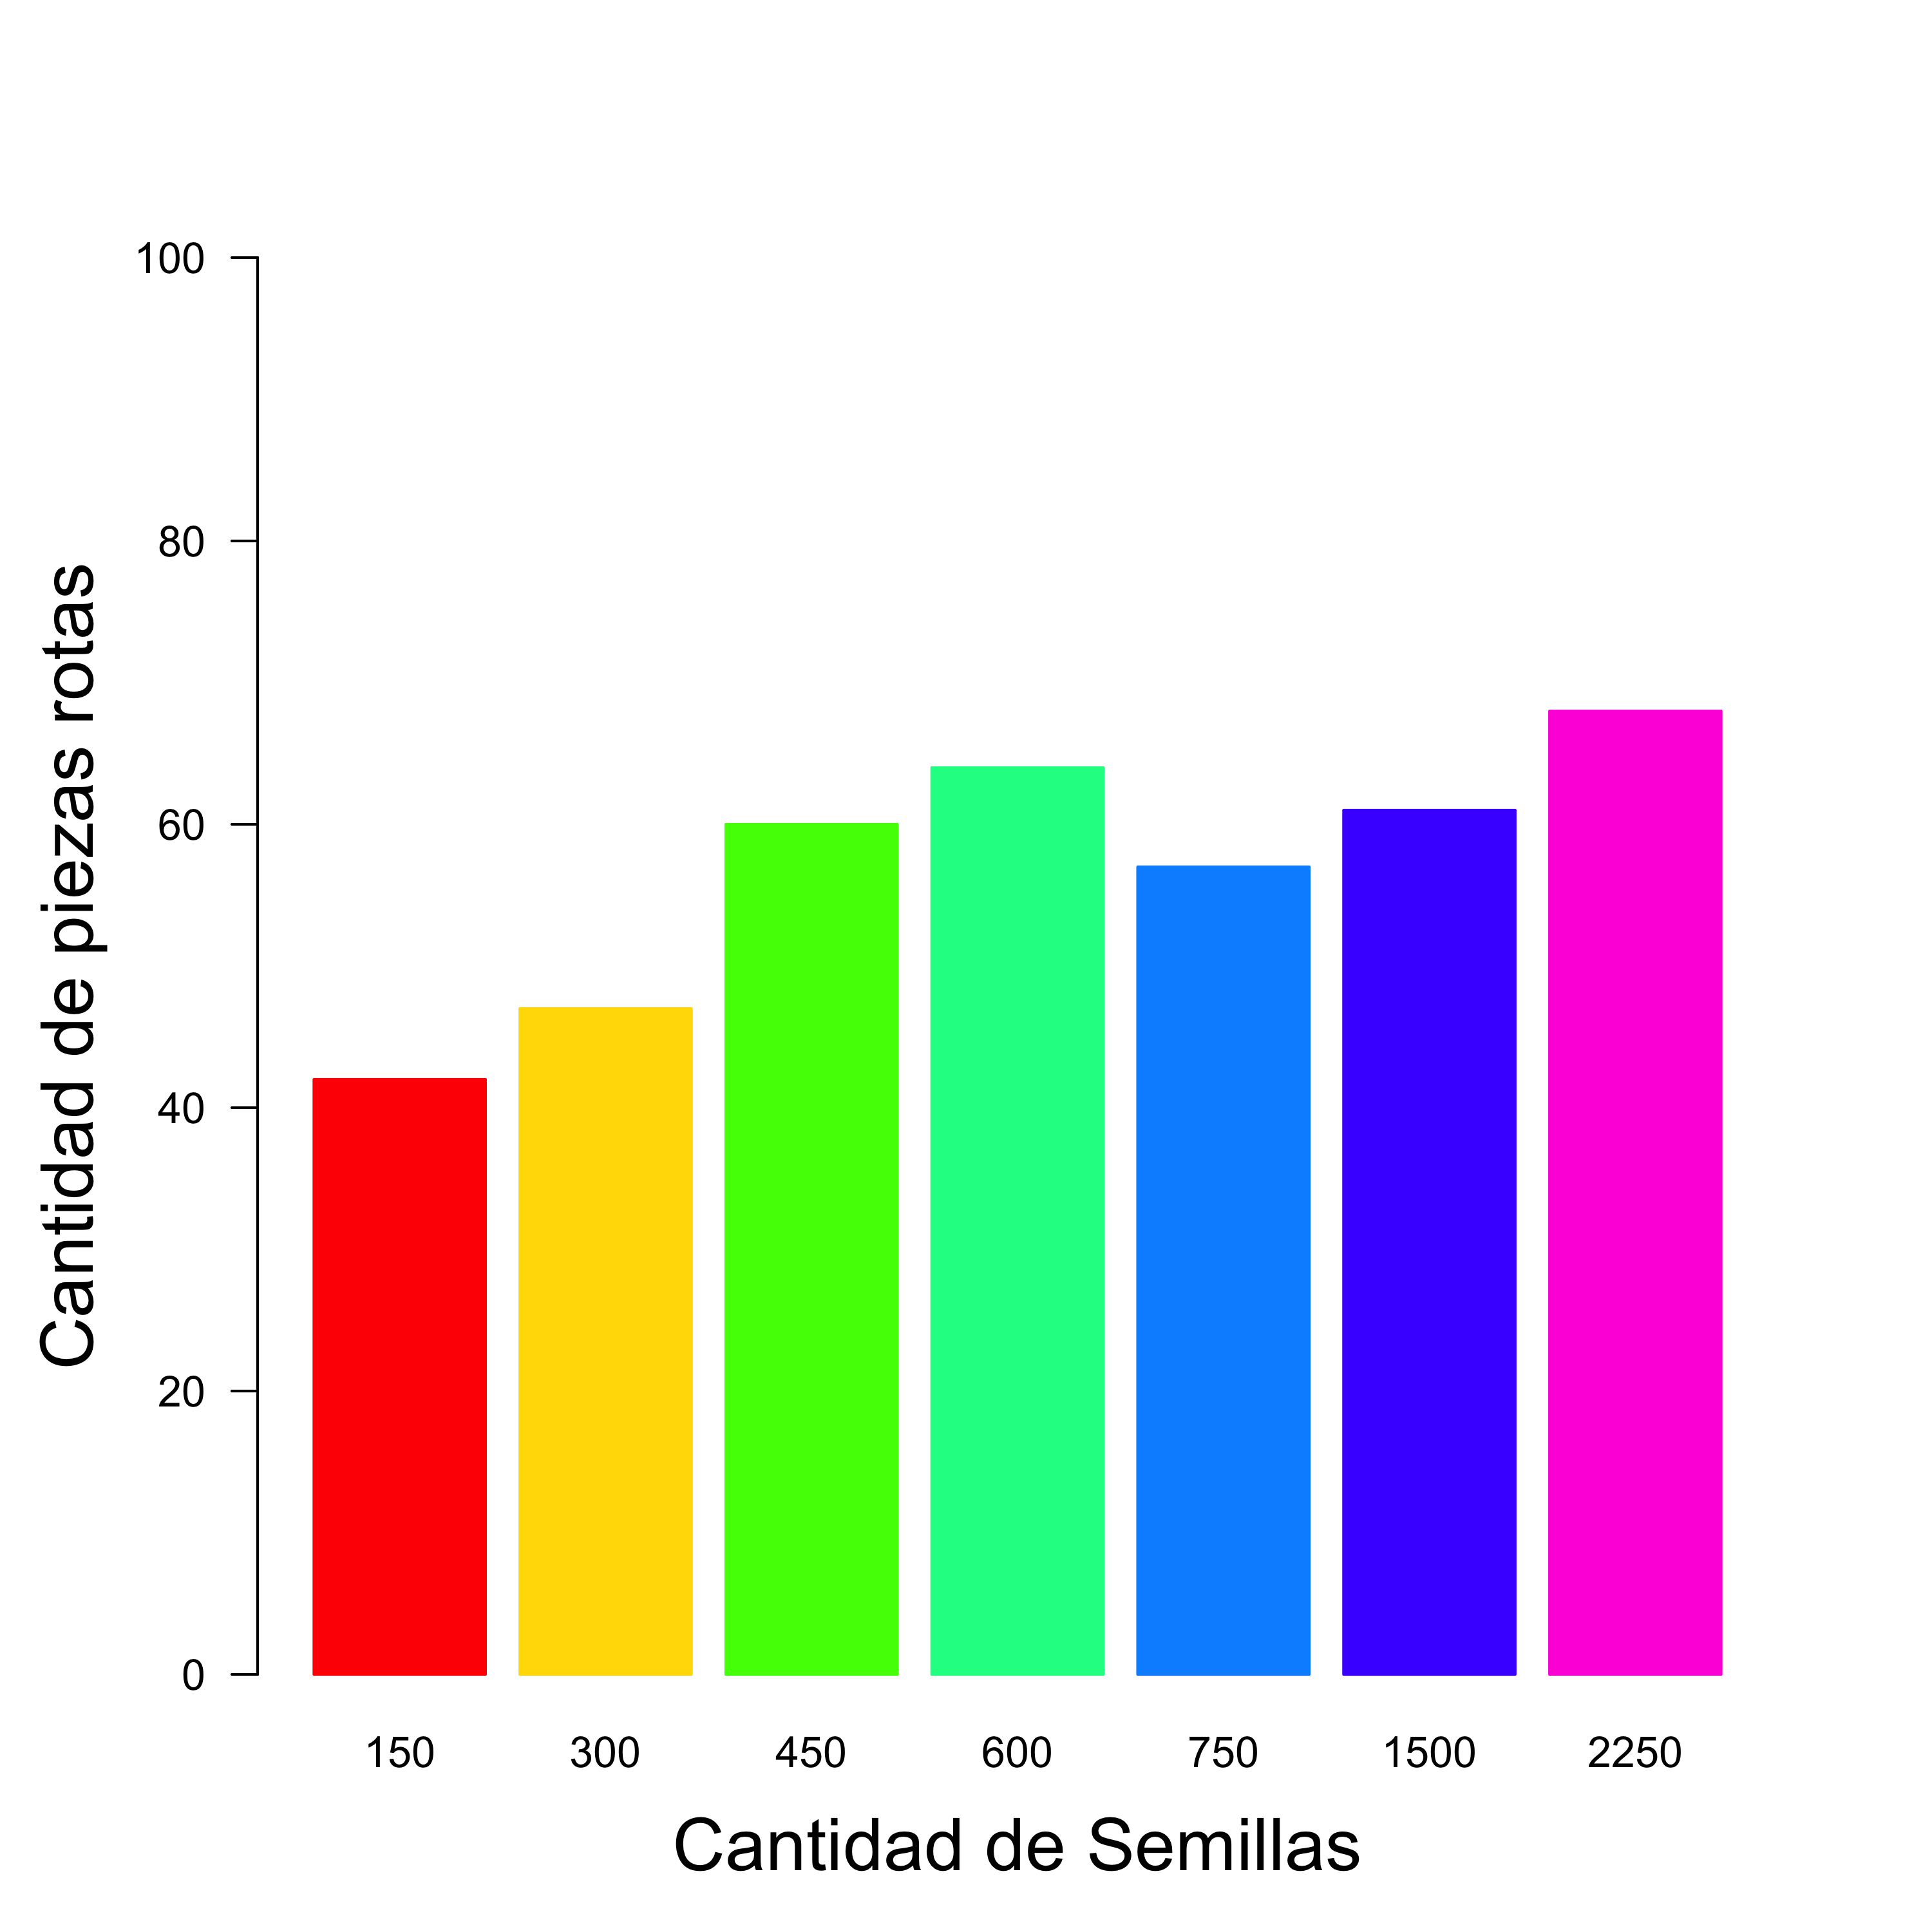
\includegraphics[width=\linewidth]{75.png} 		
 		\caption{Subconjunto con el 75\% del frente original.}
 		\label{75}
 	\end{subfigure} 
 	 	\label{por}
 	\caption{Variando el tamaño del subconjunto (naranja) del frente de Pareto (morado).}
\end{figure} 
\bibliographystyle{plain} 
\bibliography{Referencias}


\end{document} 